\documentclass[12pt,a4paper]{article}
\usepackage[width=.75\textwidth]{caption}
\usepackage{graphicx}
\usepackage{authblk}
\usepackage{amsmath}
\usepackage[top=2cm, bottom=2cm, left=2cm, right=2cm]{geometry}
\usepackage{fancyhdr}

\pagestyle{fancy}
\begin{document}

%title and author details
\title{The Unruh Effect as Holographic Thrust}
\author[1]{Kevin Player\footnote{kjplaye@gmail.com}}

\maketitle

\abstract{We outline the holographic scenario in \cite{entropic} and additionally consider the dynamics of the holographic screen itself in an accelerating frame.  We consider the case where the screen's acceleration is due to mass/energy joining with the screen, increasing the entropy of the screen.  From this we derive the Unruh effect \cite{unruh} using both classical and quantum techniques.}

\section{The Holographic Scenario}
We first recall the setup outlined in \cite{entropic}. Consider a holographic screen with entropy $S$.  Let there be a test particle which is a single wavelength $\Delta x$ away from $S$.  Following Bekenstein, we can regard the particle to be simultanously near and on the screen.

Let the screen have energy $E_S$ and mass $M_S$.  Suppose that the holographic screen is being propelled by a stream of photons in place of the test particle.  We want to see how the dynamics of the photons affects the dynamics and information carried by the screen.

\begin{figure}[h]
\centering
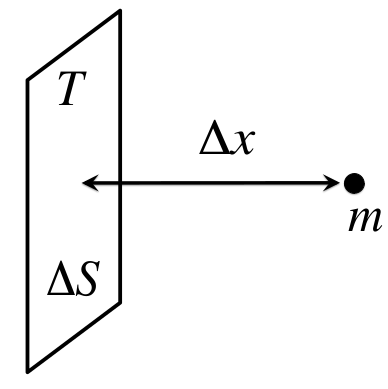
\includegraphics[scale=1.2]{screen.png}
\caption{This figure was copied from \cite{entropic}.  A test particle with mass $m$ and Compton wavelength $\Delta x$ is being absorbed into the holographic screen.  In this note, we replace the test particle with a single photon.}
\label{fig:x cubed graph}
\end{figure}
There are some complementary notions of ``emergence'' that we inherit from \cite{entropic}.  A third notion, item 3, that we supply here is the time-reversal of matter/energy emerging from the screen.
\begin{enumerate}
  \item The usual thermodynamic emergence of macrostate variables (such as temperature) from microstate variables (energies of individual particles).  This includes the emergence of Newton's laws and entropic gravity.
  \item The emergence of ``new'' space-time beyond holographic screens, treating screens like stretched horizons.  The existence of a foliation of screens where test particles move from screen to screen.
  \item Known matter/energy in front of the screen passes to unknown matter/energy on the screen. The matter/energy in front of the screen has known information.  When passing into the screen, the information is thermalized, and becomes unknown.
\end{enumerate}
The information theoretic notions of emergence will be discussed in more detail in terms of Landauer's language in the next section.

\section{Landauer Limit}
We want to keep track of the information corresponding to degrees of freedom on the screen. It is interesting to compare this situation with the limiting case of Landauer \cite{landauer}.  The situation is identical, the holographic screen in his case is the separation between the system and the heat bath (between the known and the unknown).  Forgetting (or learning) information is the same thing as letting the information ``join the screen''.

We pause to note that there is nothing canonical about choosing a bit to express this information.  For instance, Landauer considered logical gates and as an example, we briefly consider the AND gate on two unbiased bits of input.  The output is a bit, but it is biased, and so it carries less than one bit of information.  The AND gate actually forgets more than a bit\footnote{It actually forgets around 1.19 bits}.  All of this is to say that the choice of $\Delta S$ is far from obvious.

Consider the case where a single photon of energy $E_p$ is joining the screen.  The change of information, per photon, will be a constant.  It is not given by $ln(2)k$, from a bit, but by another number
\[
  \Delta S = 4 \pi ^ 2 k.
\]
There is nothing mysterious here, we pick this constant so that we will match the constant in Unruh radiation. All of the dimensional analysis will also be seen to match up and be motivated in the next section.  We leave in universal constants mainly for context.

\section{Unruh Effect Classical Derivation}

We will derive the Unruh temperature equation from the information change of an accelerating screen using the thrust of photons. For a single photon, consider the Planck relation for the energy and frequency of the screen
\[
  E_S = h f_S = \frac{h}{\Delta t}
\]
where $\Delta t$ is the period of $S$. Let $a$ be the acceleration due to the photon which we also write as $a = \Delta v / \Delta t$.  Let $p$ be the momentum of the photon, $E_p$ its energy, and we equate the momenta $p_S$ = $p_p$ = $p$.  Then
\[
  a M_S \Delta t = M_S  \Delta v = p = E_p / c
  \]
and setting a temperature $T$, with respect to $E_p$, we get
\[
  \frac{4 \pi^2 k}{h} E_S = \frac{\Delta S}{\Delta t} = \frac{E_p}{T \Delta t} = \frac{ca M_S}{T} = \frac{aE_S}{cT}
\]
and canceling $E_S$ we derive the Unruh temperature \cite{unruh}
\[
T = \frac{h}{4\pi^2k c} a
\]

\section{Hawking-Bekenstein Radiation}

The equivalence principle allows us to derive a temperature for acceleration due to gravity near the event horizon of a black hole.  This corresponds to a reference frame which continues to thrust away from a black hole maintaining a given height.  Much like the Unruh radiation, we find this thrust accounts for Hawking-Bekenstien radiation.

\section{Field Theoretic Considerations}
TODO - SHOW THAT THE UNRUH MODES COME ALTERNATIVELY AS AN INHOMOGENEOUS KLIEN-GORDON EQUATION TERM WHICH IS DRIVEN AS AN EXTERNAL SOURCE (THRUST)
\cite{beisert}


NOTE: The source can come from a term, $\rho \phi$, added to the Lagrangian.


MORE NOTES FOLLOW. The Rindler/Unruh modes can be decomposed into functions of $u = z-t$ and of $v = z+t$.  These are extensions of the future, $u=0$, and past, $v=0$, event horizons for the $z>|t|$ Rindler wedge.  The unnormalized modes are $u^{iw}$ and $v^{iw}$ and a certain linear combination of these, for each positive $\omega$, gives analytic continuations of the Rindler modes to full Minkowski space.  The strength and details of this combination lead to the celebrated expectation of Unruh particles.

The Fourier transform of these event horizon modes, when $\omega > 0$, is given for $u$ by
\[
\begin{aligned}
\int_0^\infty         & e^{-i p u} u^{i\omega} du &=&             &(i p)^{-(1 + i\omega)}\Gamma(1 + i\omega)              & = a_\omega p^{-(1 + i\omega)} \\
\int_{-\infty}^0       & e^{-i p u} u^{i\omega} du &=& e^{-\pi\omega}&(-i p)^{-(1 + i\omega)}\Gamma(1 + i\omega) & = b_\omega p^{-(1 + i\omega)} \\
\int_{-\infty}^\infty   & e^{-i p u} u^{i\omega} du & &            & (a_\omega + b_\omega) p^{-(1 + i\omega)}               & = c_\omega p^{-(1 + i\omega)} \\
\end{aligned}
\]
where the first line assumes $Im(p) < 0$, the second line assumes $Im(p) > 0$ and the third line {\bf is a lie :P}

We end up with a mode $\rho(p)$

CITE WOLFRAM ALPHA and maybe do the standard QFT contour integral trick(s) to make it not a lie.

FINALLY, TRY TO USE THE MODES AS DRIVING SOURCES OF THE INHOMOGENOUS KLIEN-GORDON EQUATION.  This seems to lead to infrared problems.  We end up with divergent integrals like this computation of expected particle number \cite{Frodden}
\[
 \int_{-\infty}^\infty \frac {|\rho(p)|^2}{2p} dp = \int_{-\infty}^\infty p^{-3} dp
\]
Which converges at $\pm \infty$ but diverges at $p=0$.

 
HOW DO WE SALVAGE THIS?


\section{Prediction}
If we do not account for the thrust required to accelerate a detector, then we recover it instead as a thermal unknown in the the vacuum.  It would seem that we can explain Unruh radiation instead using thrust and basic holographic information theoretic arguments alone.  LINK IN QFT SECTION. The prediction of this note is that Unruh radiation, separate from thrust, should not appear.

\begin{thebibliography}{2}

\bibitem{beisert}
Niklas Beisert notes, last section of 
https://edu.itp.phys.ethz.ch/hs12/qft1/Chapter03.pdf
FIX UP THIS ENTRY

\bibitem{bekenstein} J. D. Bekenstein, “Black holes and entropy,” Phys. Rev. D 7, 2333 (1973).

\bibitem{Frodden}
E.~Frodden and N.~Vald\'es,
``UNRUH EFFECT: Introductory Notes to Quantum Effects for Accelerated Observers,''
Int. J. Mod. Phys. A \textbf{33}, no.27, 1830026 (2018)
doi:10.1142/S0217751X18300260
[arXiv:1806.11157 [gr-qc]].
  
\bibitem{landauer}
Rolf Landauer (1961), "Irreversibility and heat generation in the computing process" (PDF), IBM Journal of Research and Development, 5 (3): 183–191, doi:10.1147/rd.53.0183, retrieved 2015-02-18.

\bibitem{unruh}
W. G. Unruh, “Notes on black hole evaporation,” Phys. Rev. D 14, 870 (1976).

\bibitem{entropic}
E.P. Verlinde (2011). "On the Origin of Gravity and the Laws of Newton". JHEP. 2011 (4): 29. arXiv:1001.0785. Bibcode:2011JHEP...04..029V. doi:10.1007/JHEP04(2011)029. S2CID 3597565.
\end{thebibliography}


\end{document}

